\documentclass{article}
\usepackage[MeX]{polski}
\usepackage[utf8]{inputenc}
\usepackage{enumerate}
\usepackage[pdftex]{graphicx} 
\author{P.Matuszak}
\title{E-Sport jako forma sportu}
\frenchspacing
\begin{document}
\maketitle
\section{Wprowadzenie}
\subsection{Co to E-Sport?}
E-Sport (pol. Sport elektroniczny) to forma rywalizacji, w której przedmiotem działań zawodników są gry komputerowe. Rywalizacja między zawodnikami odbywa się zarówno w formie rekreacyjnej, jak i na turniejach gier komputerowych. Mecze rozgrywane są na żywo, a publiczność może oglądać graczy siedzących przed komputerami, zaś ich posunięcia śledzić na wielkich telebimach. Rozgrywki w internecie są wykorzystywane częściej przy eliminacjach. Formuła sportu elektronicznego przyciąga coraz większe rzesze graczy w wieku od kilku do kilkudziesięciu lat, głównie dzięki niwelowaniu barier fizycznych, spotykanych w sporcie tradycyjnym, przy jednoczesnym zachowaniu poczucia rywalizacji sportowej.
\subsection{Historia E-Sportu}
Historia e-sportu wiąże się ze wzrastającą popularnością rozgrywek sieciowych w grach takich jak StarCraft, Counter-Strike, Quake, Warcraft II: Tides of Darkness czy League of Legends. Popularność Quake'a przyczyniła się do powstania w 1997 roku w Stanach Zjednoczonych ligi zawodowych graczy Cyberathlete Professional League. Na świecie działają objęte prestiżem turnieje takie jak World Cyber Games i Electronic Sports World Cup, a w Polsce – Poznań Game Arena oraz Electronic Sports League. Poszczególne gry komputerowe różnych gatunków, w których toczy się rozgrywka między zawodnikami, są nazywane dyscyplinami.
\section{Polska w E-Sporcie}
\subsection{Counter Strike Global Offensive}
Virtus.pro to zespół grający dla rosyjskiej organizacji, choć w jego skład wchodzą sami Polacy. Dlatego też Virtus.pro uważa się za polski zespół. Jest to jeden z najlepszych zespół na scenie CS GO. Do zespołu należą:\\
\begin{tabular}{|c|c|c|c|} \hline
Nick & Imie i nazwisko & Wiek & Miasto\\
\hline
Byali & Paweł Bieliński & 19 lat & Szczecin\\
\hline
Neo & Filip Kubski & 26 lat & Poznań\\
\hline
Pasha & Jarosław Jarząbkowski & 25 lat & Waszawa\\
\hline
Snax & Janusz Pogorzelski & 20 lat & Kraków\\
\hline
TaZ & Wiktor Wojtas & 27 lat & Warszawa\\
\hline
\end{tabular}\\ \\
Każdy gracz potrzebuje sprzętu, dlatego poniżej zamieszam listę z wyposażeniem graczy:
\begin{enumerate}
  \item Byali
  \begin{enumerate}
    \item Mysz: Steelseries Kinzu v3
    \item Podkładka: Steelseries Qck
    \item Klawiatura: Steelseries 6gv2
    \item Słuchawki: Qpad QH-1339
  \end{enumerate}
  \item Neo
  \begin{enumerate}
    \item Mysz: Zowie FK1 Pro
    \item Podkładka: Zowie CM
    \item Klawiatura: Tesoro Colada Evil
    \item Słuchawki: Qpad QH-90
  \end{enumerate}
  \item Pasha
  \begin{enumerate}
    \item Mysz: Steelseries Kinzu v3
    \item Podkładka: Qpad UC
    \item Klawiatura: Tesoro Colada Saint
    \item Słuchawki: Qpad QH-1339
  \end{enumerate}
  \item SnaX
  \begin{enumerate}
    \item Mysz: Zowie FK1 Pro
    \item Podkładka: Roccat Taito king Size
    \item Klawiatura: Tesoro Durandal Ultimate
    \item Słuchawki: Steelseries Siberia v3
  \end{enumerate}
  \item TaZ
  \begin{enumerate}
    \item Mysz: Zowie EC1`
    \item Podkładka: Qpad UC
    \item Klawiatura: Tesoro Colada Saint
    \item Słuchawki: Qpad QH-1339
  \end{enumerate}
\end{enumerate}
\subsection{League of Legends}
League of Legends to sieciowa gra komputerowa z gatunku multiplayer online battle arena. Powstała na bazie modyfikacji Defense of the Ancients (DotA) do Warcraft III: The Frozen Throne. Została opracowana przez Riot Games i początkowo wydana tylko dla systemu Windows. Po raz pierwszy ogłoszona 7 października 2008, a wydana 27 października 2009, 15 lipca 2013 gra została uznana w USA za pełnoprawny sport.\\
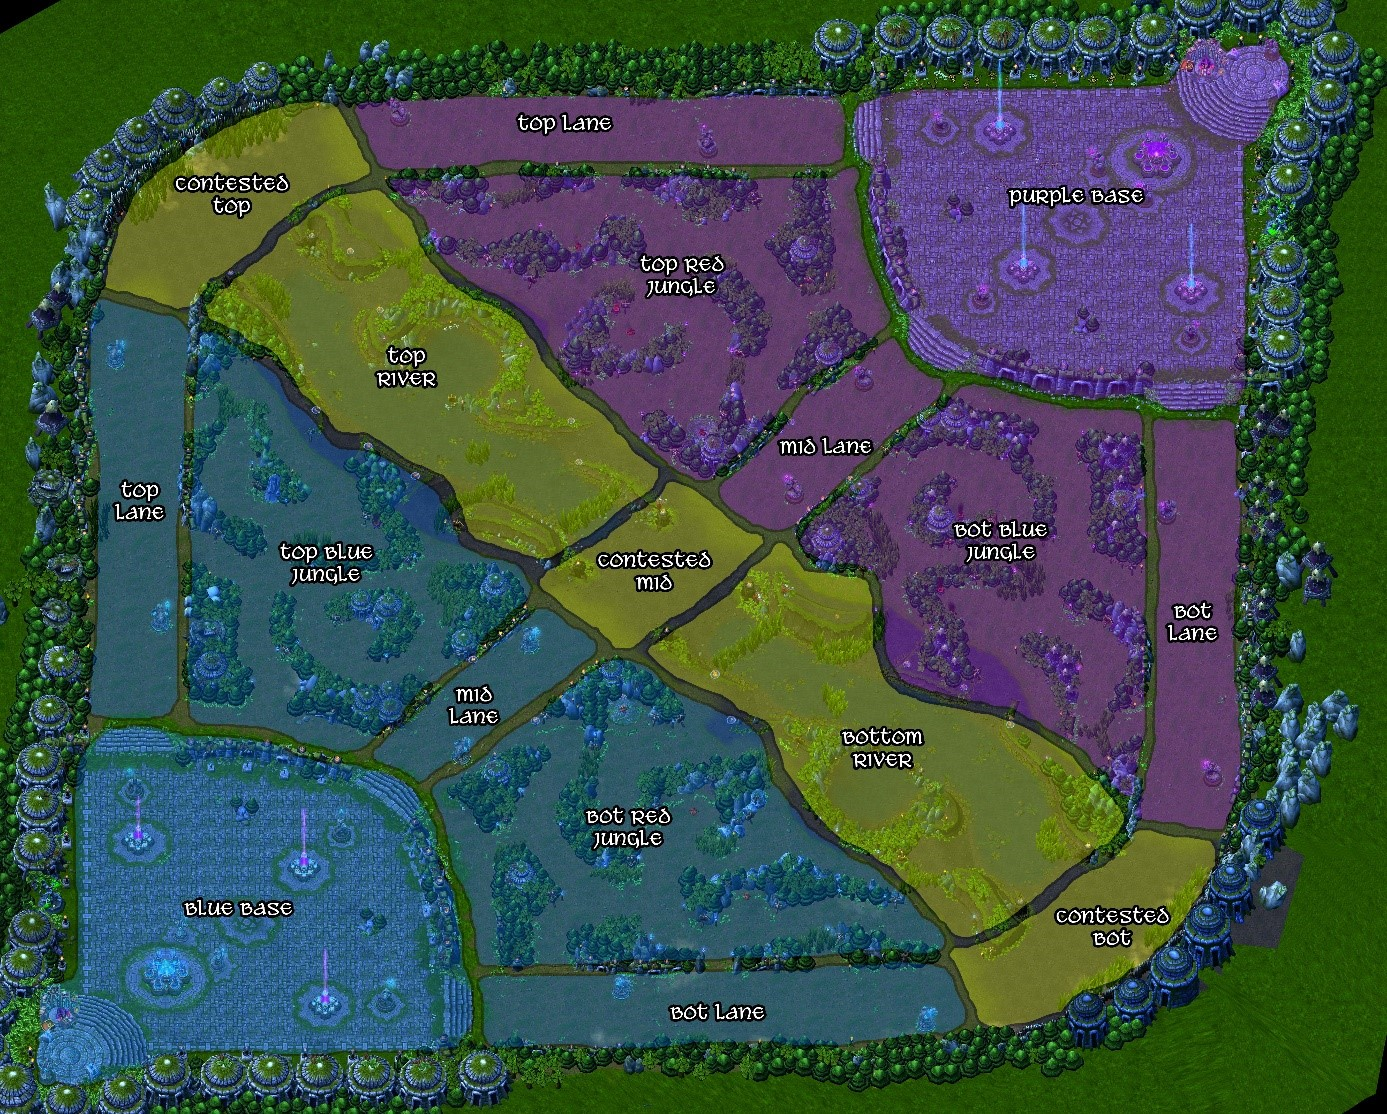
\includegraphics[width=3cm]{mapa}
\end{document}